\chapter{Interconnected: a working prototype}
This chapter discusses the creation of a working prototype that realizes a subset of core functionalities of the system. Firstly, the goals and context for the prototype are discussed. Then, the simplified architecture for the prototype is presented, providing also details on the realization of the single entities that compose such architecture. The third section will then contain a brief explanation of the setup related to DevOps methodologies. After that, the Coordination section will talk about the messages exchanged between the entities in order to realize the desired functionalities. Concluding this chapter, the simplified Proto-MapReduce implementation realized will be discussed and, after that, data regarding real-world experiments will be presented. 

\section{Goals and context}
After having engineered a complete system that satisfies the use cases defined in \textit{section \ref{use_cases}}, it is now time to create a prototype that brings a portion of it to reality. The prototype takes the name of the "Interconnected project".

Before explaining the work behind this prototype, a few premises have to be clarified in order to understand some choices taken during the development.

Firstly, the focus of this work is to discuss the topic of integrating mobile devices in a Grid system and, most importantly, engineering a solution that defines a blueprint for actually bringing the idea to reality. Due to a lack of resources (economical, time, equipment, team members, etc...), the prototype does not try to realize the whole system defined in the previous chapter, but only a subset of core functionalities with the goal to demonstrate that the core idea is also technologically feasible.

As a direct consequence of that, the prototype will not realize aspects that, while certainly important in a real product, do possess already well-established technologies (authentication, data storage, server instances replication, payment systems, etc...), focusing only on the innovative aspects of the project.

\section{Simplified architecture}
\textit{Figure \ref{fig:simplified_architecture}} shows a complete view of the entities composing the simplified architecture for the Interconnected project (that can be compared to the full architecture shown in \textit{figure \ref{fig:architecture_complete}}).

\begin{figure}[!ht]
    \centering
    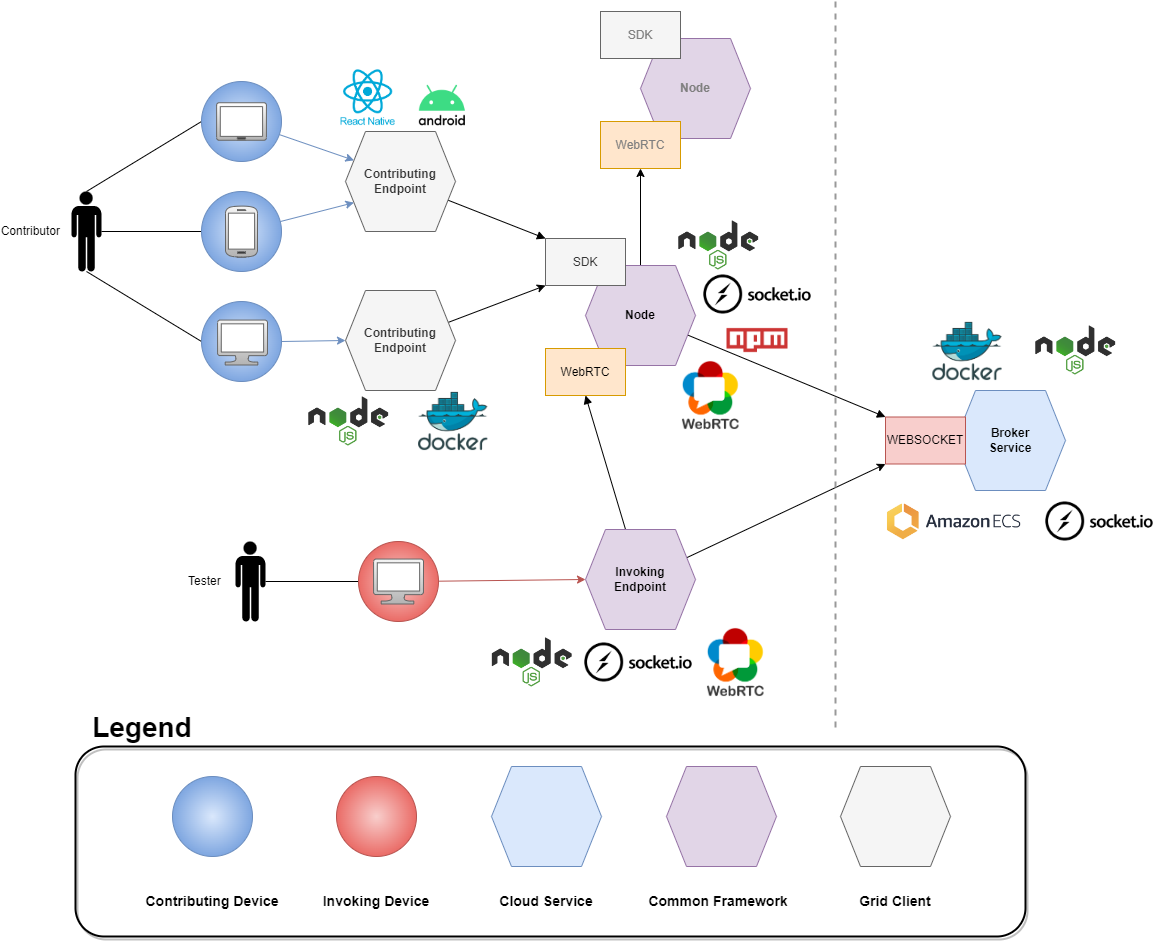
\includegraphics[width=\linewidth]{document/chapters/chapter_7/images/simplified_architecture.png}
    \caption{Complete view of the simplified prototype's architecture}
    \label{fig:simplified_architecture}
\end{figure}

\vspace{10mm}

All the entities composing the architecture are implemented using technologies based on Node.js which offers useful, popular and well maintained frameworks as well as an easy to use concurrency model based on an event loop.

\subsection{Broker Service}
TODO technologies and stuff

The only Cloud Service present is the Broker Service; since only one instance (with a static address) of such Cloud Service is required to sustain the workload of the few devices connected, a dynamic handling and discovery of multiple instances is thus not required. As a direct consequence of that, the complementary entities that handled the dynamic system for scalability (Grid Master Service, Broker Discovery Service and Grid Services Gateway Service) are not needed and thus Nodes and Invoking Endpoints communicate directly with the Broker Service without first undergoing the discovery processes described in \textit{section \ref{use_cases_satisfaction}}.

\subsection{Interconnected Node}
TODO technologies and stuff

The Node entity concretizes its P2P connectivity requirements through the use of the WebRTC (Real-Time Communication for the Web) protocol; such communication standard it is used to send audio and video data among peers, as well as any kind of structured non-media data. In order for the peers to establish the connection, first the signaling process needs to be completed: the peers, through a third intermediary (the Broker Service), exchange some information required for the connection to happen; the Peer that initializes the connection creates an SDP (Signaling Description Protocol) object, denominated "offer". When the other Peer receives such data, it also creates its SDP object denominated "answer". Once each Peers posses both generated SDP data, they finalize the connection exchanging some ICE (Interactive Connectivity Establishment) candidates; such ICE candidates needs to be specified when realizing a WebRTC connection since they are the actual servers that allow the P2P connection. There are two types of servers involved:
\begin{itemize}
    \item \textbf{STUN} (Session Traversal Utilities for NAT)\\
    Used by Peers that resides behind the same NAT; through this server the IP info of each Peer are retrieved and a direct P2P connection can be established.
    \item \textbf{TURN} (Traversal Using Relays around NAT)\\
    Used by Peers that resides in different NATs; through this server the limitations of a NAT are overcome, creating an indirect P2P connection that uses the TURN server to forward the messages among the two Peers.
\end{itemize}

\begin{figure}[!ht]
    \centering
    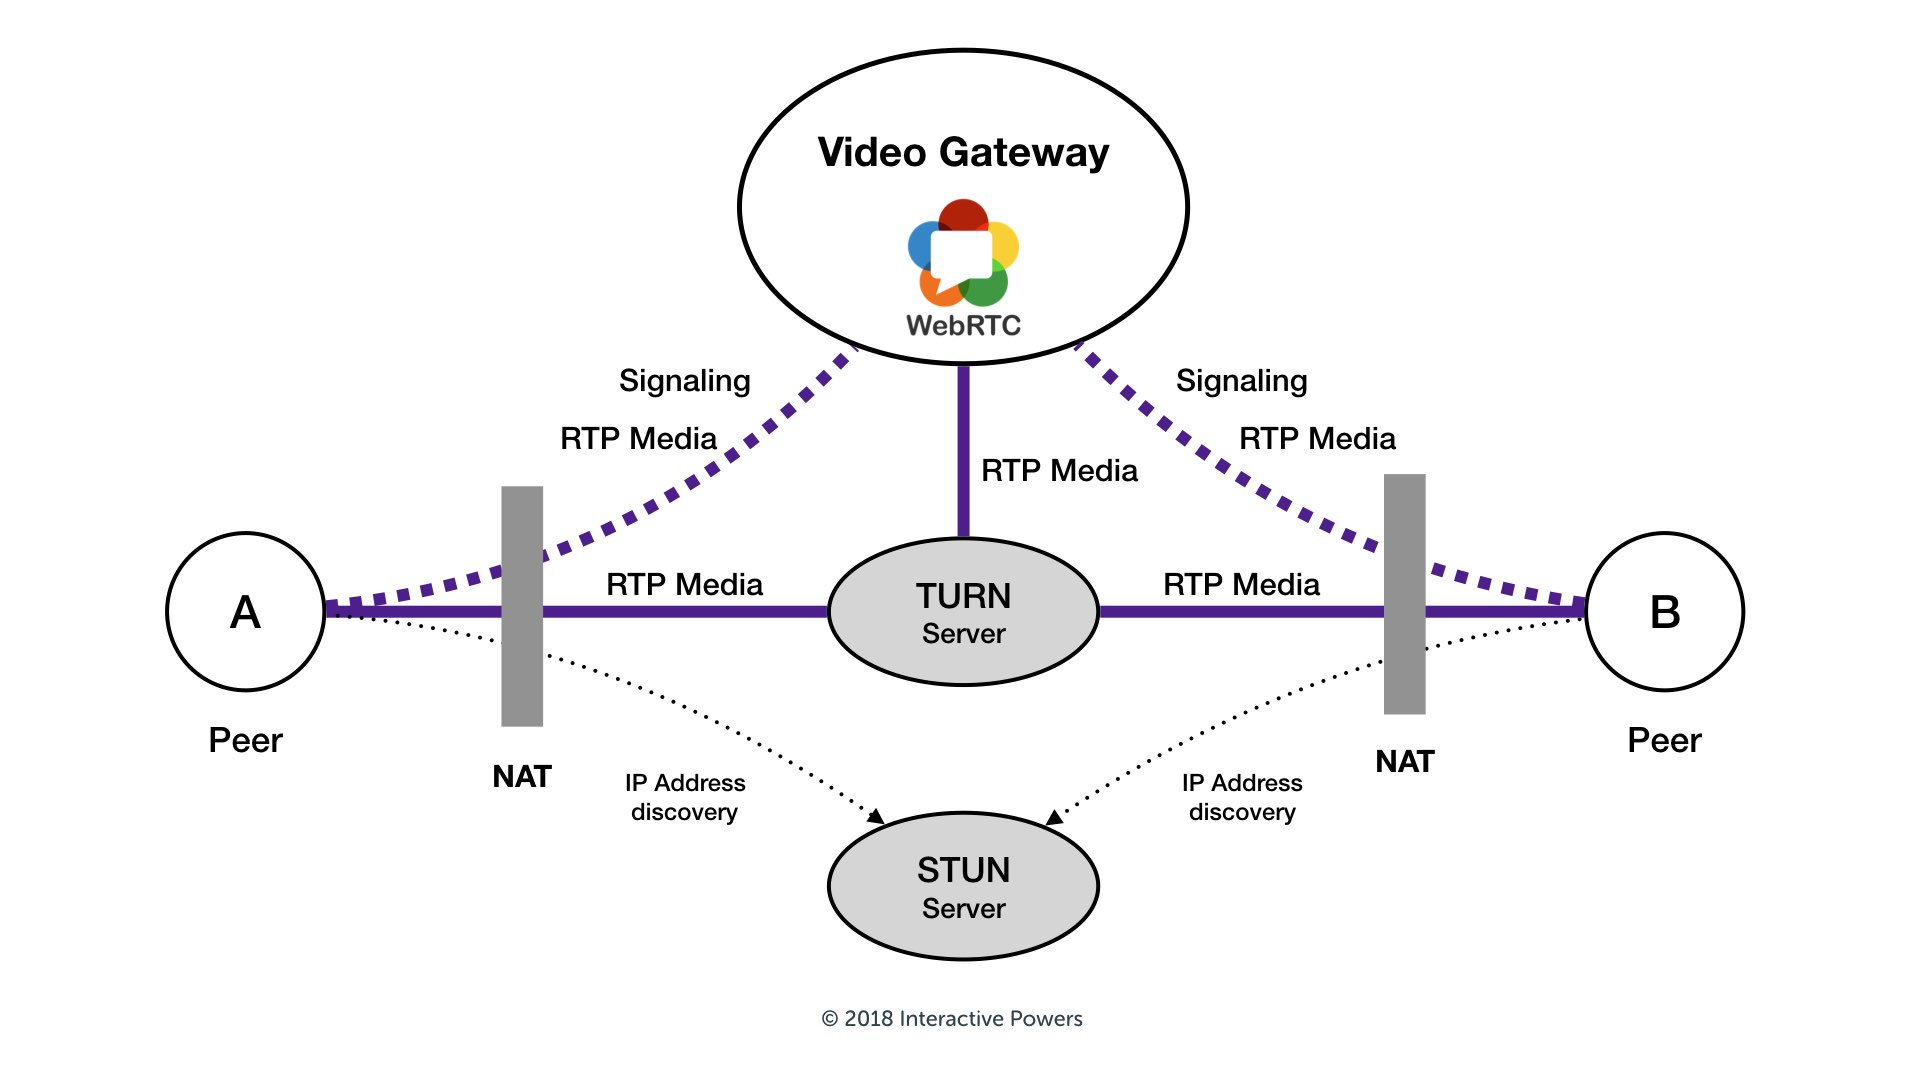
\includegraphics[width=\linewidth]{document/chapters/chapter_7/images/webrtc.jpeg}
    \caption{WebRTC - STUN and TURN servers \cite{stun_and_turn_servers}}
    \label{fig:webrtc}
\end{figure}

Free STUN and TURN servers (used by this prototype) are available thanks to the \textbf{\href{https://www.metered.ca/tools/openrelay/}{Open Relay}} initiative.

\subsection{Interconnected Mobile Client}
TODO

\begin{figure}[!ht]
    \centering
    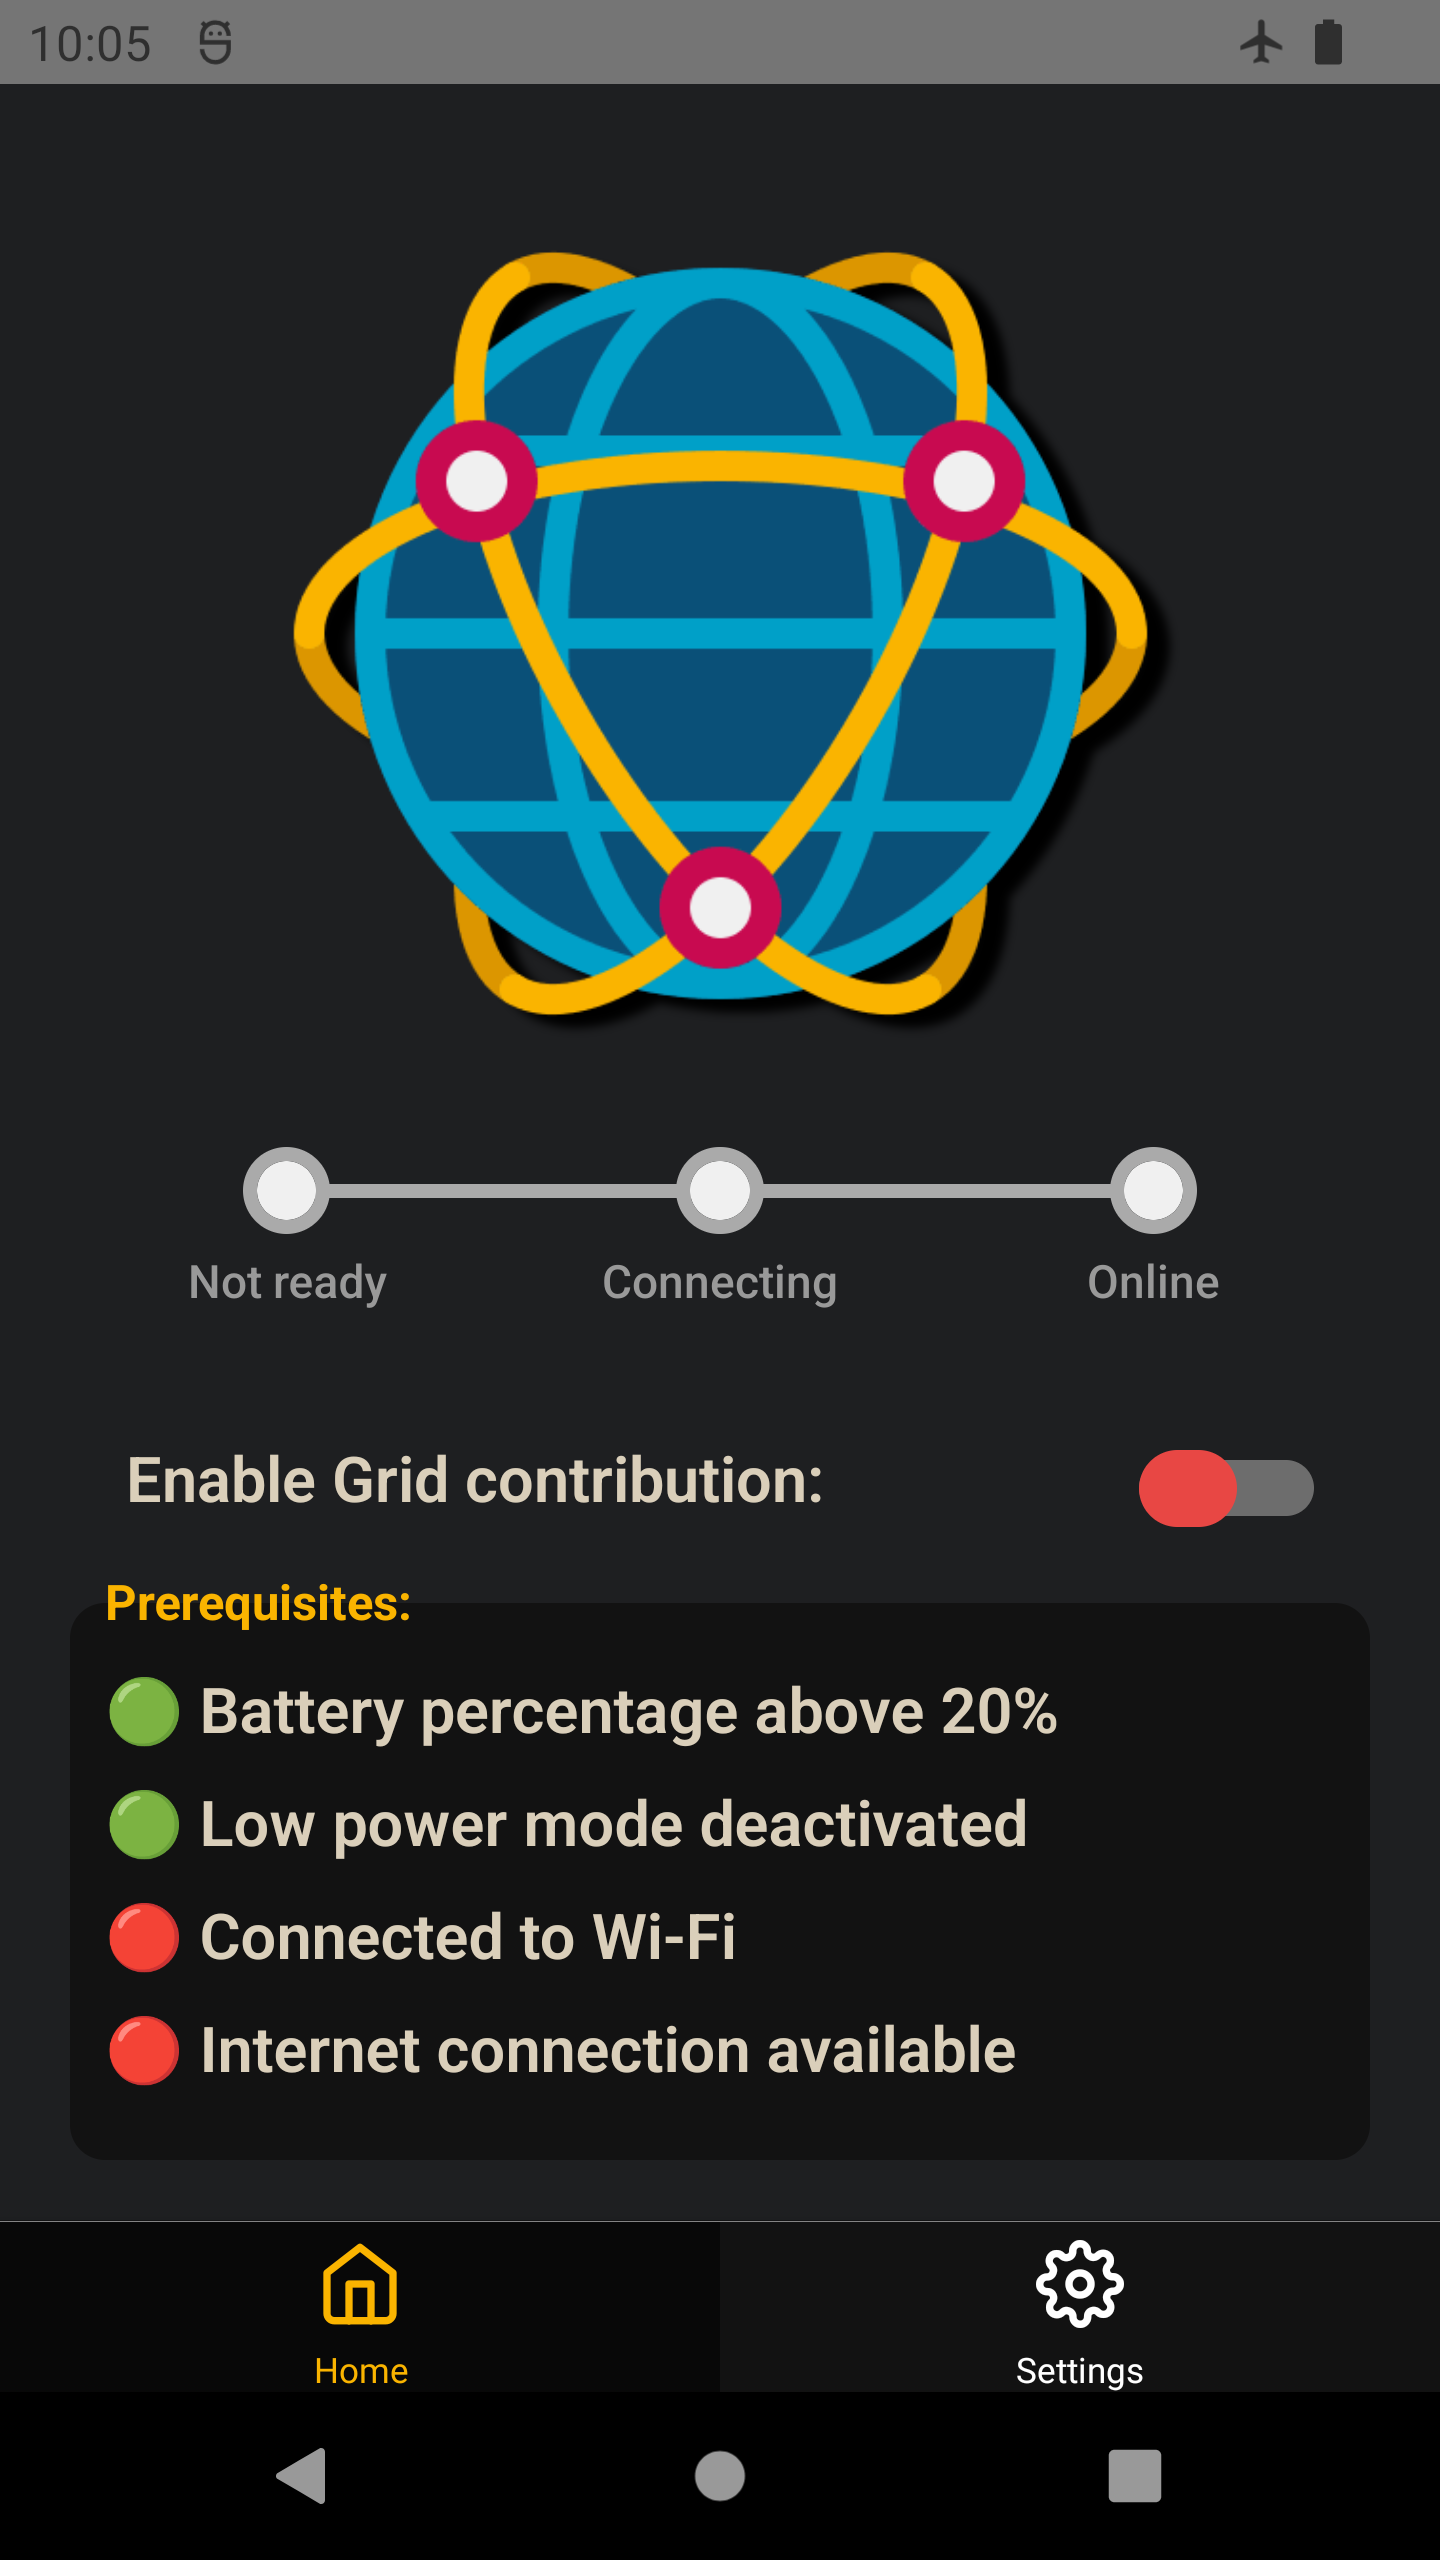
\includegraphics[scale=0.15]{document/chapters/chapter_7/images/interconnected_mobile_home.png}
    \caption{Interconnected Mobile Client}
    \label{fig:interconnected_mobile_home}
\end{figure}

\begin{figure}[!ht]
    \centering
    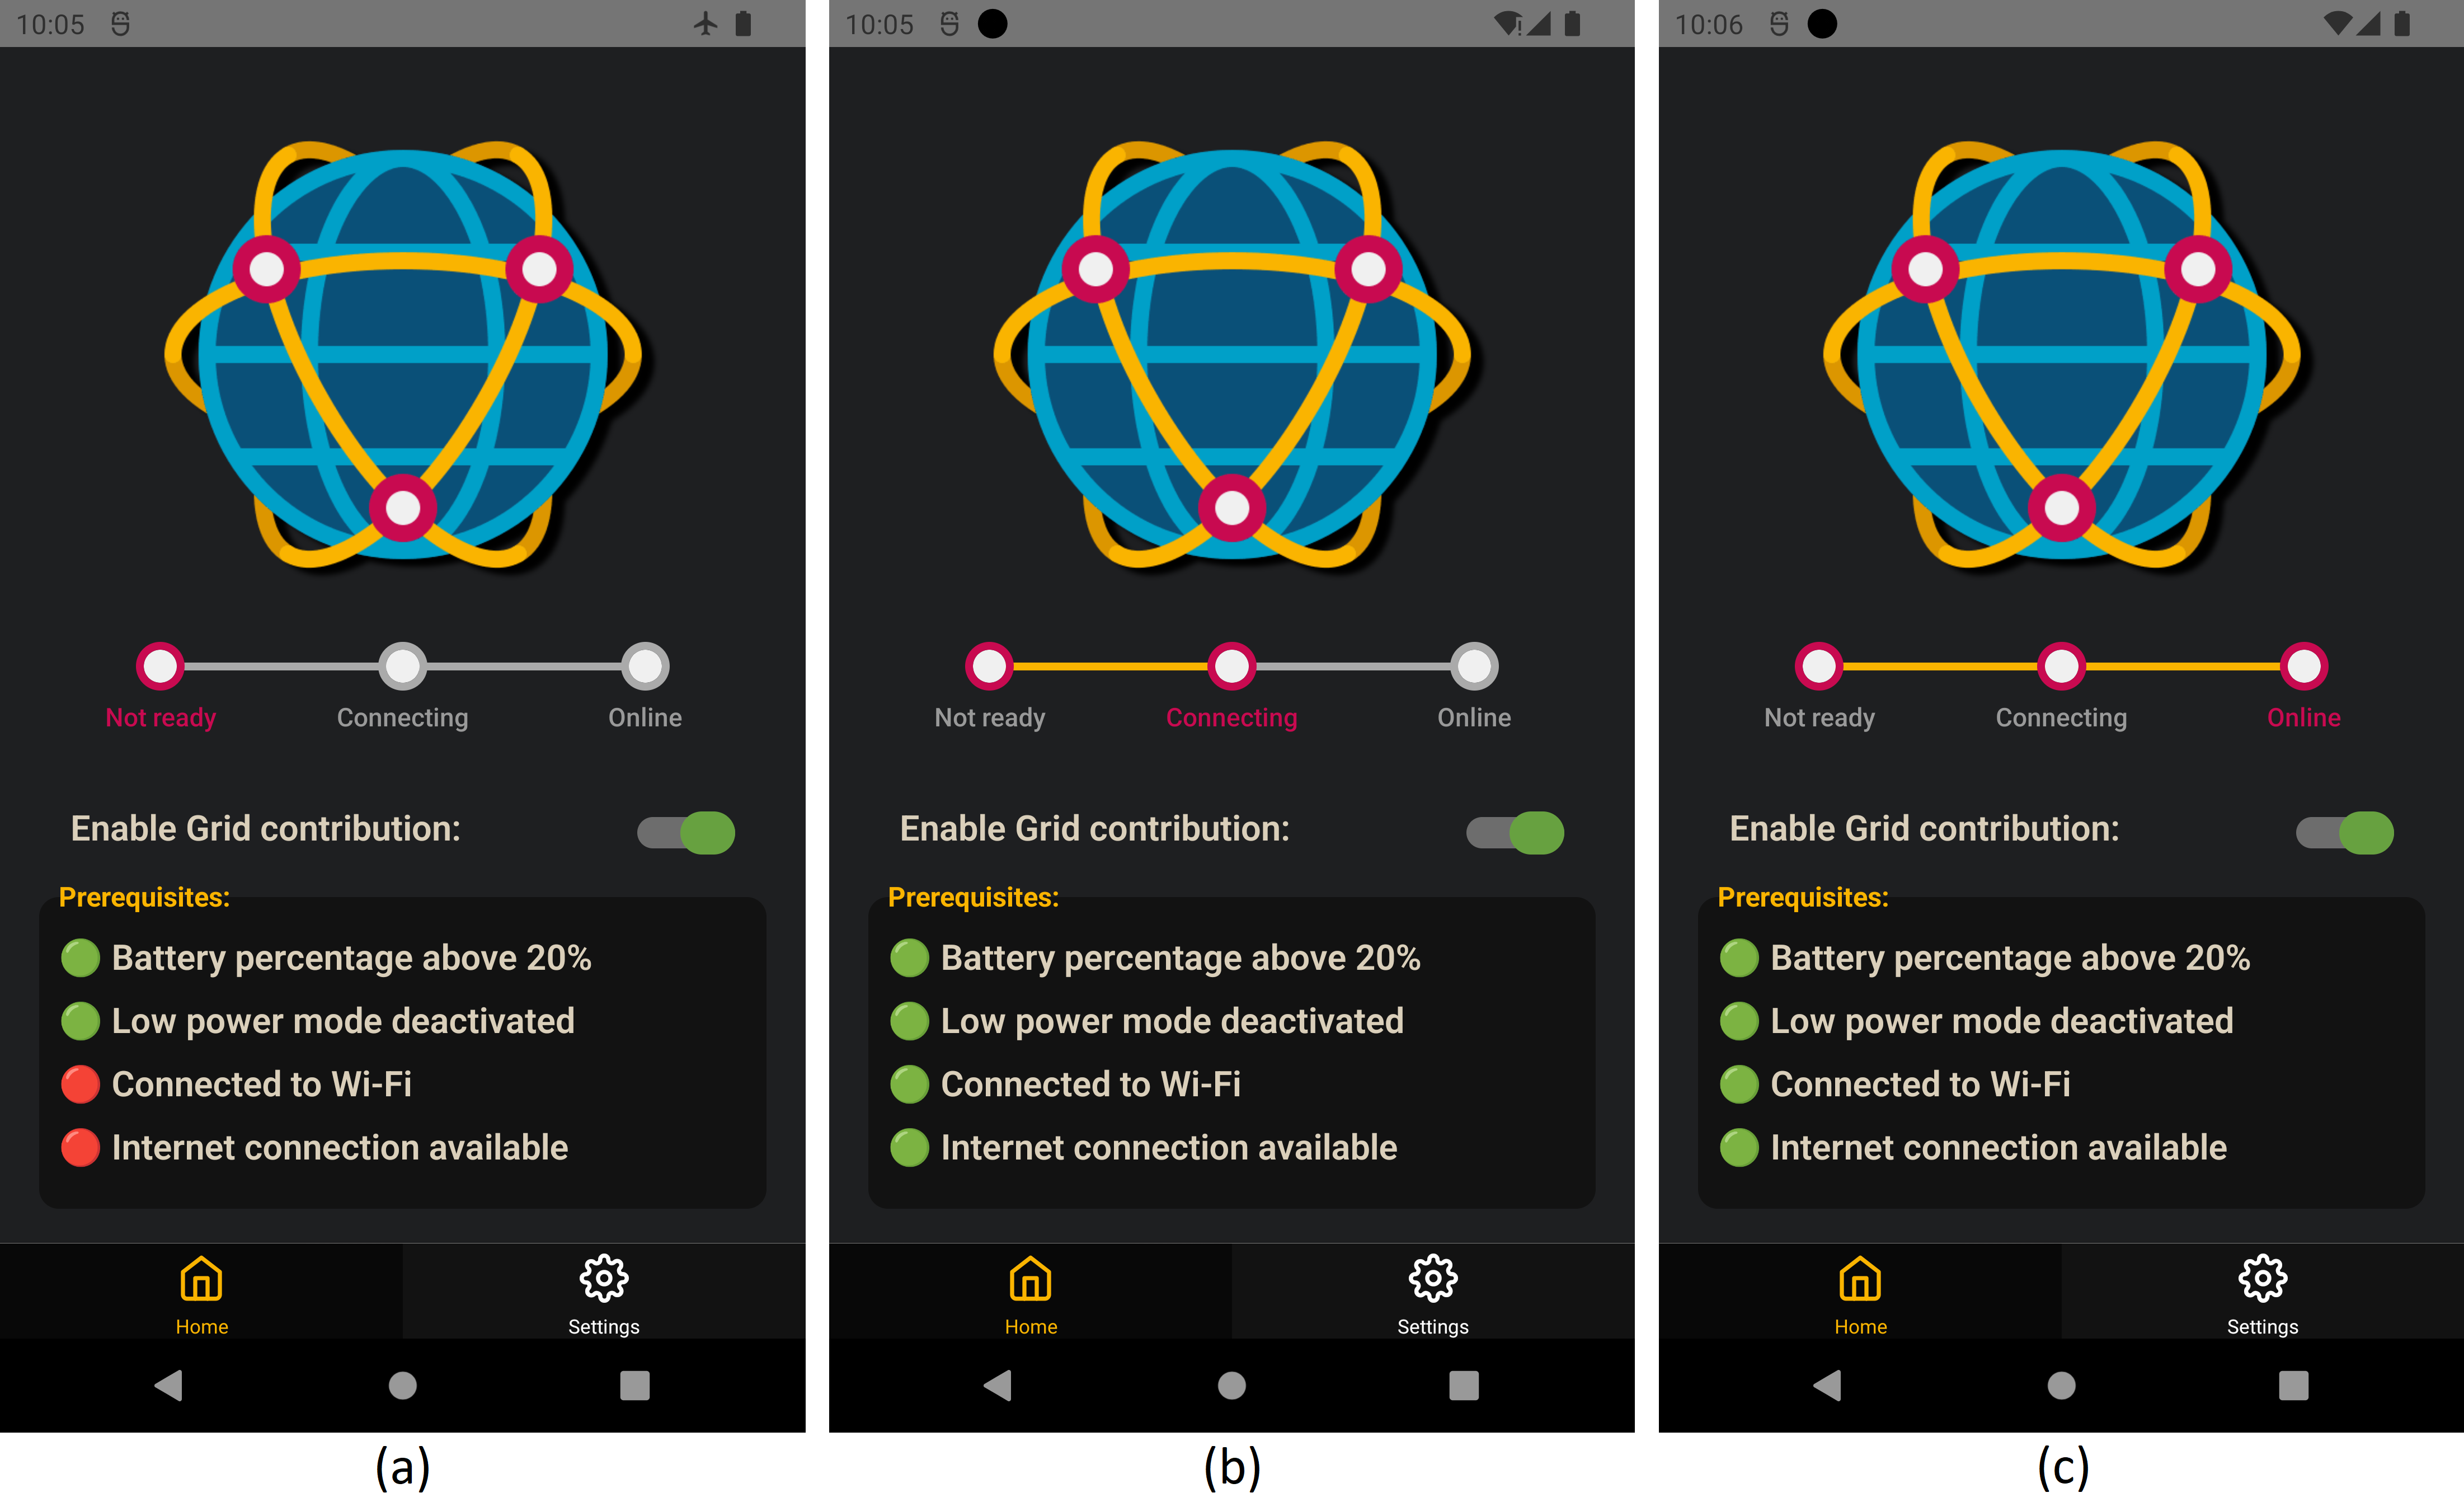
\includegraphics[width=\linewidth]{document/chapters/chapter_7/images/interconnected_mobile_connection.png}
    \caption{Interconnected Mobile Client - Connection}
    \label{fig:interconnected_mobile_connection}
\end{figure}

\begin{figure}[!ht]
    \centering
    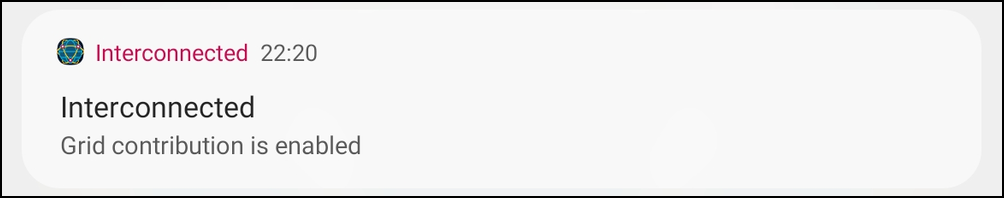
\includegraphics[scale=0.3]{document/chapters/chapter_7/images/notification_contribution.png}
    \caption{Interconnected Mobile Client - Grid contribution enabled notification}
    \label{fig:notification_contribution}
\end{figure}

\begin{figure}[!ht]
    \centering
    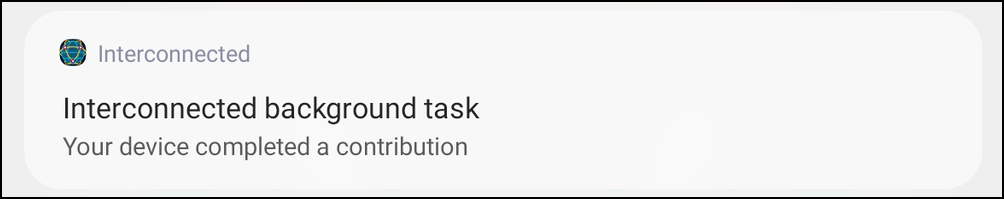
\includegraphics[scale=0.3]{document/chapters/chapter_7/images/notification_completed.png}
    \caption{Interconnected Mobile Client - Grid contribution completed notification}
    \label{fig:notification_completed}
\end{figure}

\subsection{Interconnected Desktop Client}
TODO

\begin{figure}[!ht]
    \centering
    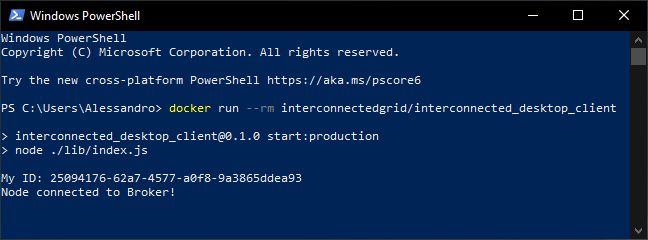
\includegraphics[scale=0.8]{document/chapters/chapter_7/images/interconnected_desktop.png}
    \caption{Interconnected Desktop Client - Docker image run on a container}
    \label{fig:interconnected_desktop}
\end{figure}

\subsection{Invoking Endpoint Prototype}
TODO
\section{DevOps}
TODO
\section{Coordination}\label{coordination}
This section analyses the \textbf{messages exchanged among the entities composing the prototype architecture}. There are \textbf{three phases} in this coordination process:
\begin{enumerate}
    \item \textbf{Grid connection}
    \item \textbf{Recruitment}
    \item \textbf{P2P messaging}
\end{enumerate}

\subsection{Grid connection}
This phase \textbf{connects a Node} (whether used by the Mobile or the Desktop client) \textbf{or an Invoking Endpoint Prototype to the Broker Service using a Socket connection} through the Socket.io framework. \textbf{The Broker Service registers the connections and uses them in the Recruitment phase}.

\subsection{Recruitment}
The recruitment phase \textbf{connects a requestor device} (that becomes the Master in the P2Pconnection) \textbf{to an actual device that will perform a Contribution} (becoming the Slave). \textbf{While a Slave is necessarily a Node, a Master can either be an Invoking Endpoint or a Node}, allowing to obtain either an \textbf{Invoking Endpoint to Node connection} or a \textbf{Node to Node connection}.

This phase is \textbf{executed exchanging messages among the soon-to-be Peers using the previously established Socket connections, but ends with a direct P2P connection} between the Master and the Slave through the WebRTC framework.

\begin{figure}[!ht]
    \centering
    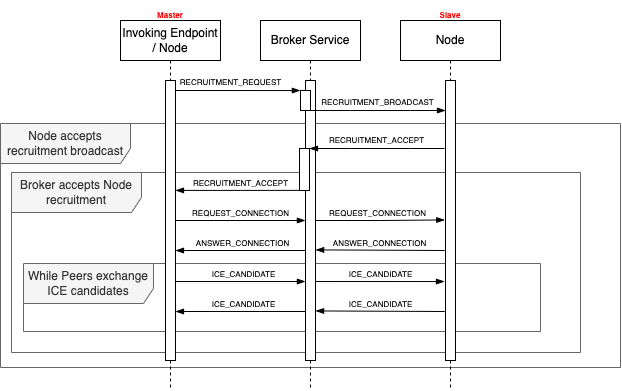
\includegraphics[scale=0.65]{document/chapters/chapter_7/images/recruitment_messages.png}
    \caption{Recruitment - Sequence Diagram}
    \label{fig:recruitment_messages}
\end{figure}

\textit{Figure \ref{fig:recruitment_messages}} shows the actual messages exchanged in this phase: the soon-to-be Master sends a \textbf{\textit{RECRUITMENT\_REQUEST}} to the Broker Service, \textbf{containing details regarding which kind of resources are needed}; the Broker Service, upon receiving this request, creates a \textbf{pending Recruitment Request} and broadcasts a \textbf{\textit{RECRUITMENT\_BROADCAST}} message to all the connected Nodes.

\textbf{The Node checks locally if it is compatible with the received request} and, if all the conditions are true, it sends a \textit{\textbf{RECRUITMENT\_ACCEPT}} message \textbf{to the Broker Service} which, upon receiving it, checks if the request is still unsatisfied, \textbf{eventually forwarding the message to the entity that first emitted the request}.

From this point on, \textbf{the P2P connection is initialized exchanging the WebRTC's required information} (previously discussed in \textit{section \ref{interconnected_node}}): the \textbf{Master} sends a \textbf{\textit{REQUEST\_CONNECTION}} message, containing its \textbf{SPD offer} and, in response, the \textbf{Slave} sends its \textbf{SDP answer} contained in a \textbf{\textit{ANSWER\_CONNECTION}} message. Once the two Peers possess each other's SDP data structures, they \textbf{start exchanging ICE candidates until they reach an agreement, finally opening the P2P connection, completing the Recruitment}.

Although the broadcast is executed once, the messages contained in the "Broker accepts Node recruitment" scope need to be exchanged every time a new P2P connection is established among two Peers.

\subsection{P2P messaging}
\textbf{Once the P2P connection is established}, \textit{figure \ref{fig:p2p_messages}} shows the \textbf{messages that the Master and the Slave exchange in their interaction}.

\begin{figure}[!ht]
    \centering
    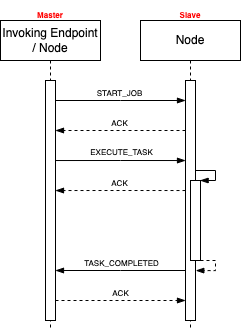
\includegraphics[scale=0.61]{document/chapters/chapter_7/images/p2p_messages.png}
    \caption{P2P messaging - Sequence Diagram}
    \label{fig:p2p_messages}
\end{figure}

\textbf{The Master sends a \textit{START\_JOB} message to the Slave}, possibly including data (which need to be sent only once) that will later be useful when executing the specific Tasks for that Job. Once the Slave has started said Job, t\textbf{he Master sends a \textbf{EXECUTE\_TASK} message}, \textbf{containing further data that}, combined with the Job's payload, \textbf{is used to perform a computation}. Upon receiving the EXECUTE\_TASK message the \textbf{Slave} sends an ACK to the Master and \textbf{enqueues the Task}, sending a \textbf{\textbf{TASK\_COMPLETED}} message (containing the result) to the Master \textbf{only when the task is actually completed}.

\textbf{This asynchronous organization allows the Master to send multiple Tasks to enqueue without waiting that the Slave has already completed its Tasks, speeding up the process}.
The Tasks submission and collection of results continues until all the Master's Tasks are completed and the P2P connection is terminated, removing the Job from the Slave.

\textbf{Using this Job/Task generalization, it is possible to construct various kinds of Grid Services}, starting from the MapReduce one.
\section{Proto-MapReduce}
TODO

\begin{figure}[!ht]
    \centering
    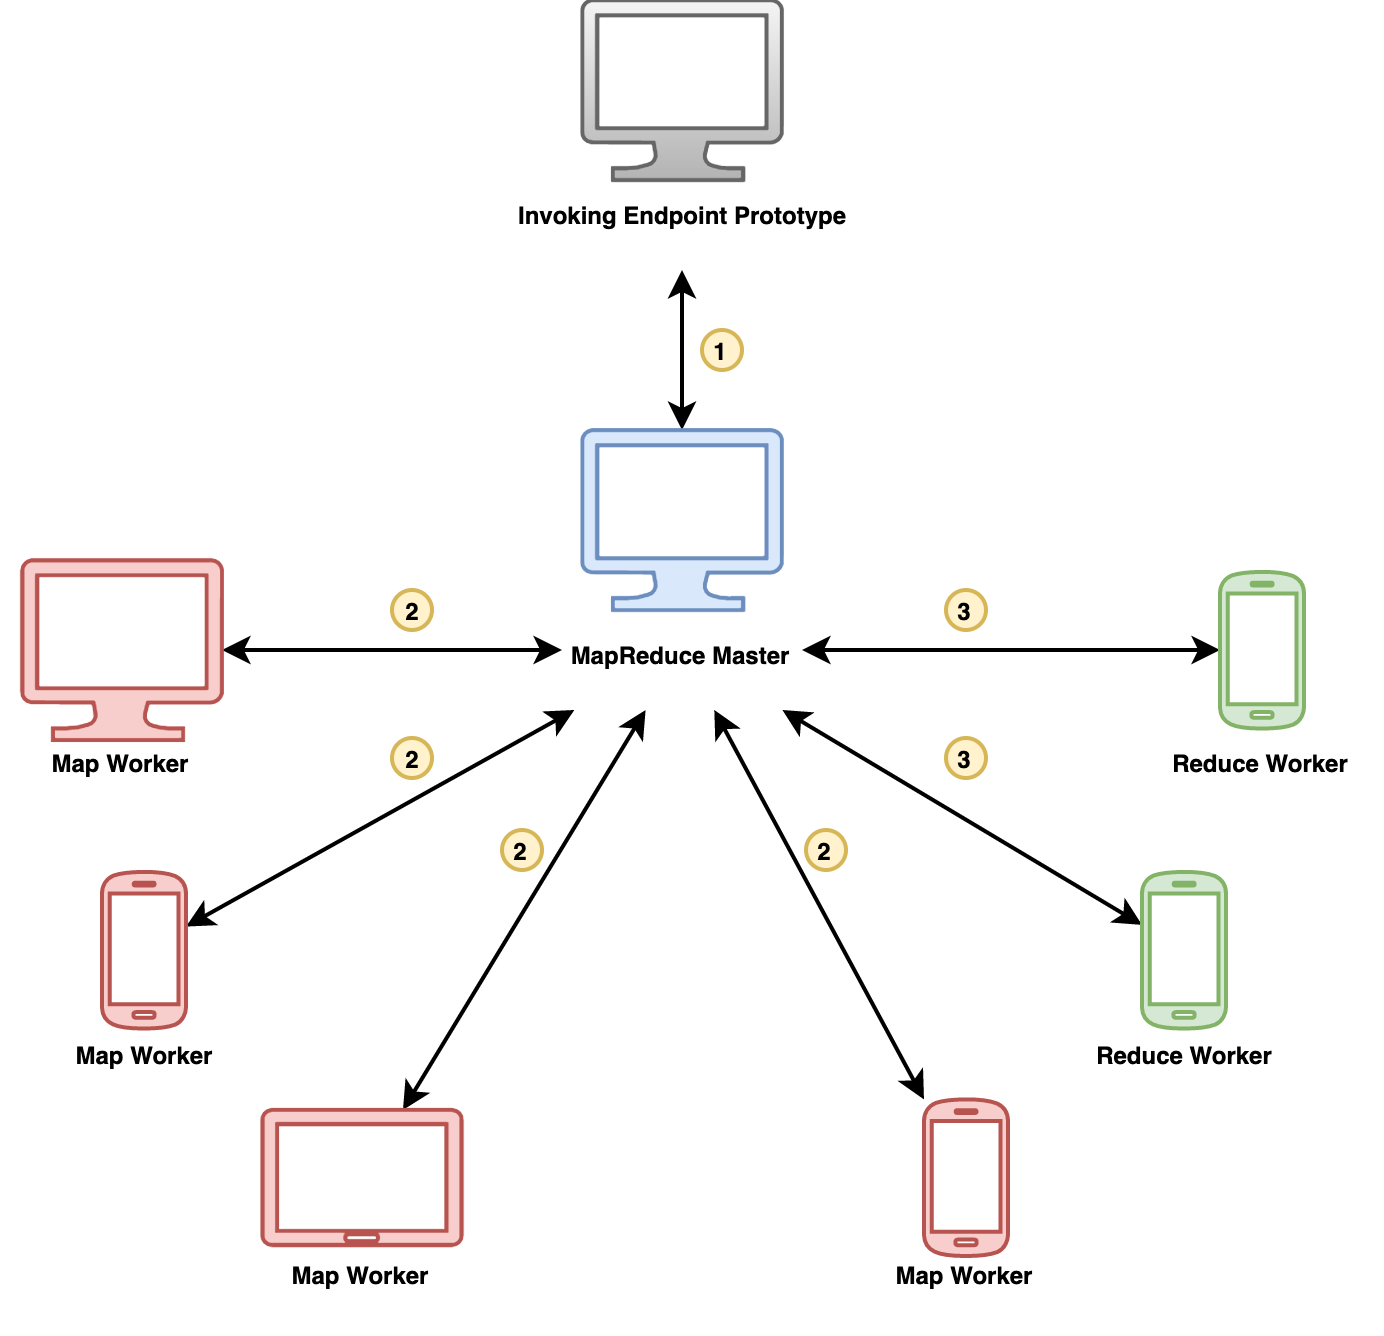
\includegraphics[scale=1.1]{document/chapters/chapter_7/images/proto_mapreduce.png}
    \caption{Proto-MapReduce Topology}
    \label{fig:proto_mapreduce}
\end{figure}
\section{Real-world experiments}\label{real_world_experiments}
This section describes the experiments performed using the prototype in a real-world scenario performing a distributed MapReduce computation on distributed heterogeneous devices.

\subsection{Computation}
TODO

\begin{figure}[!ht]
    \centering
    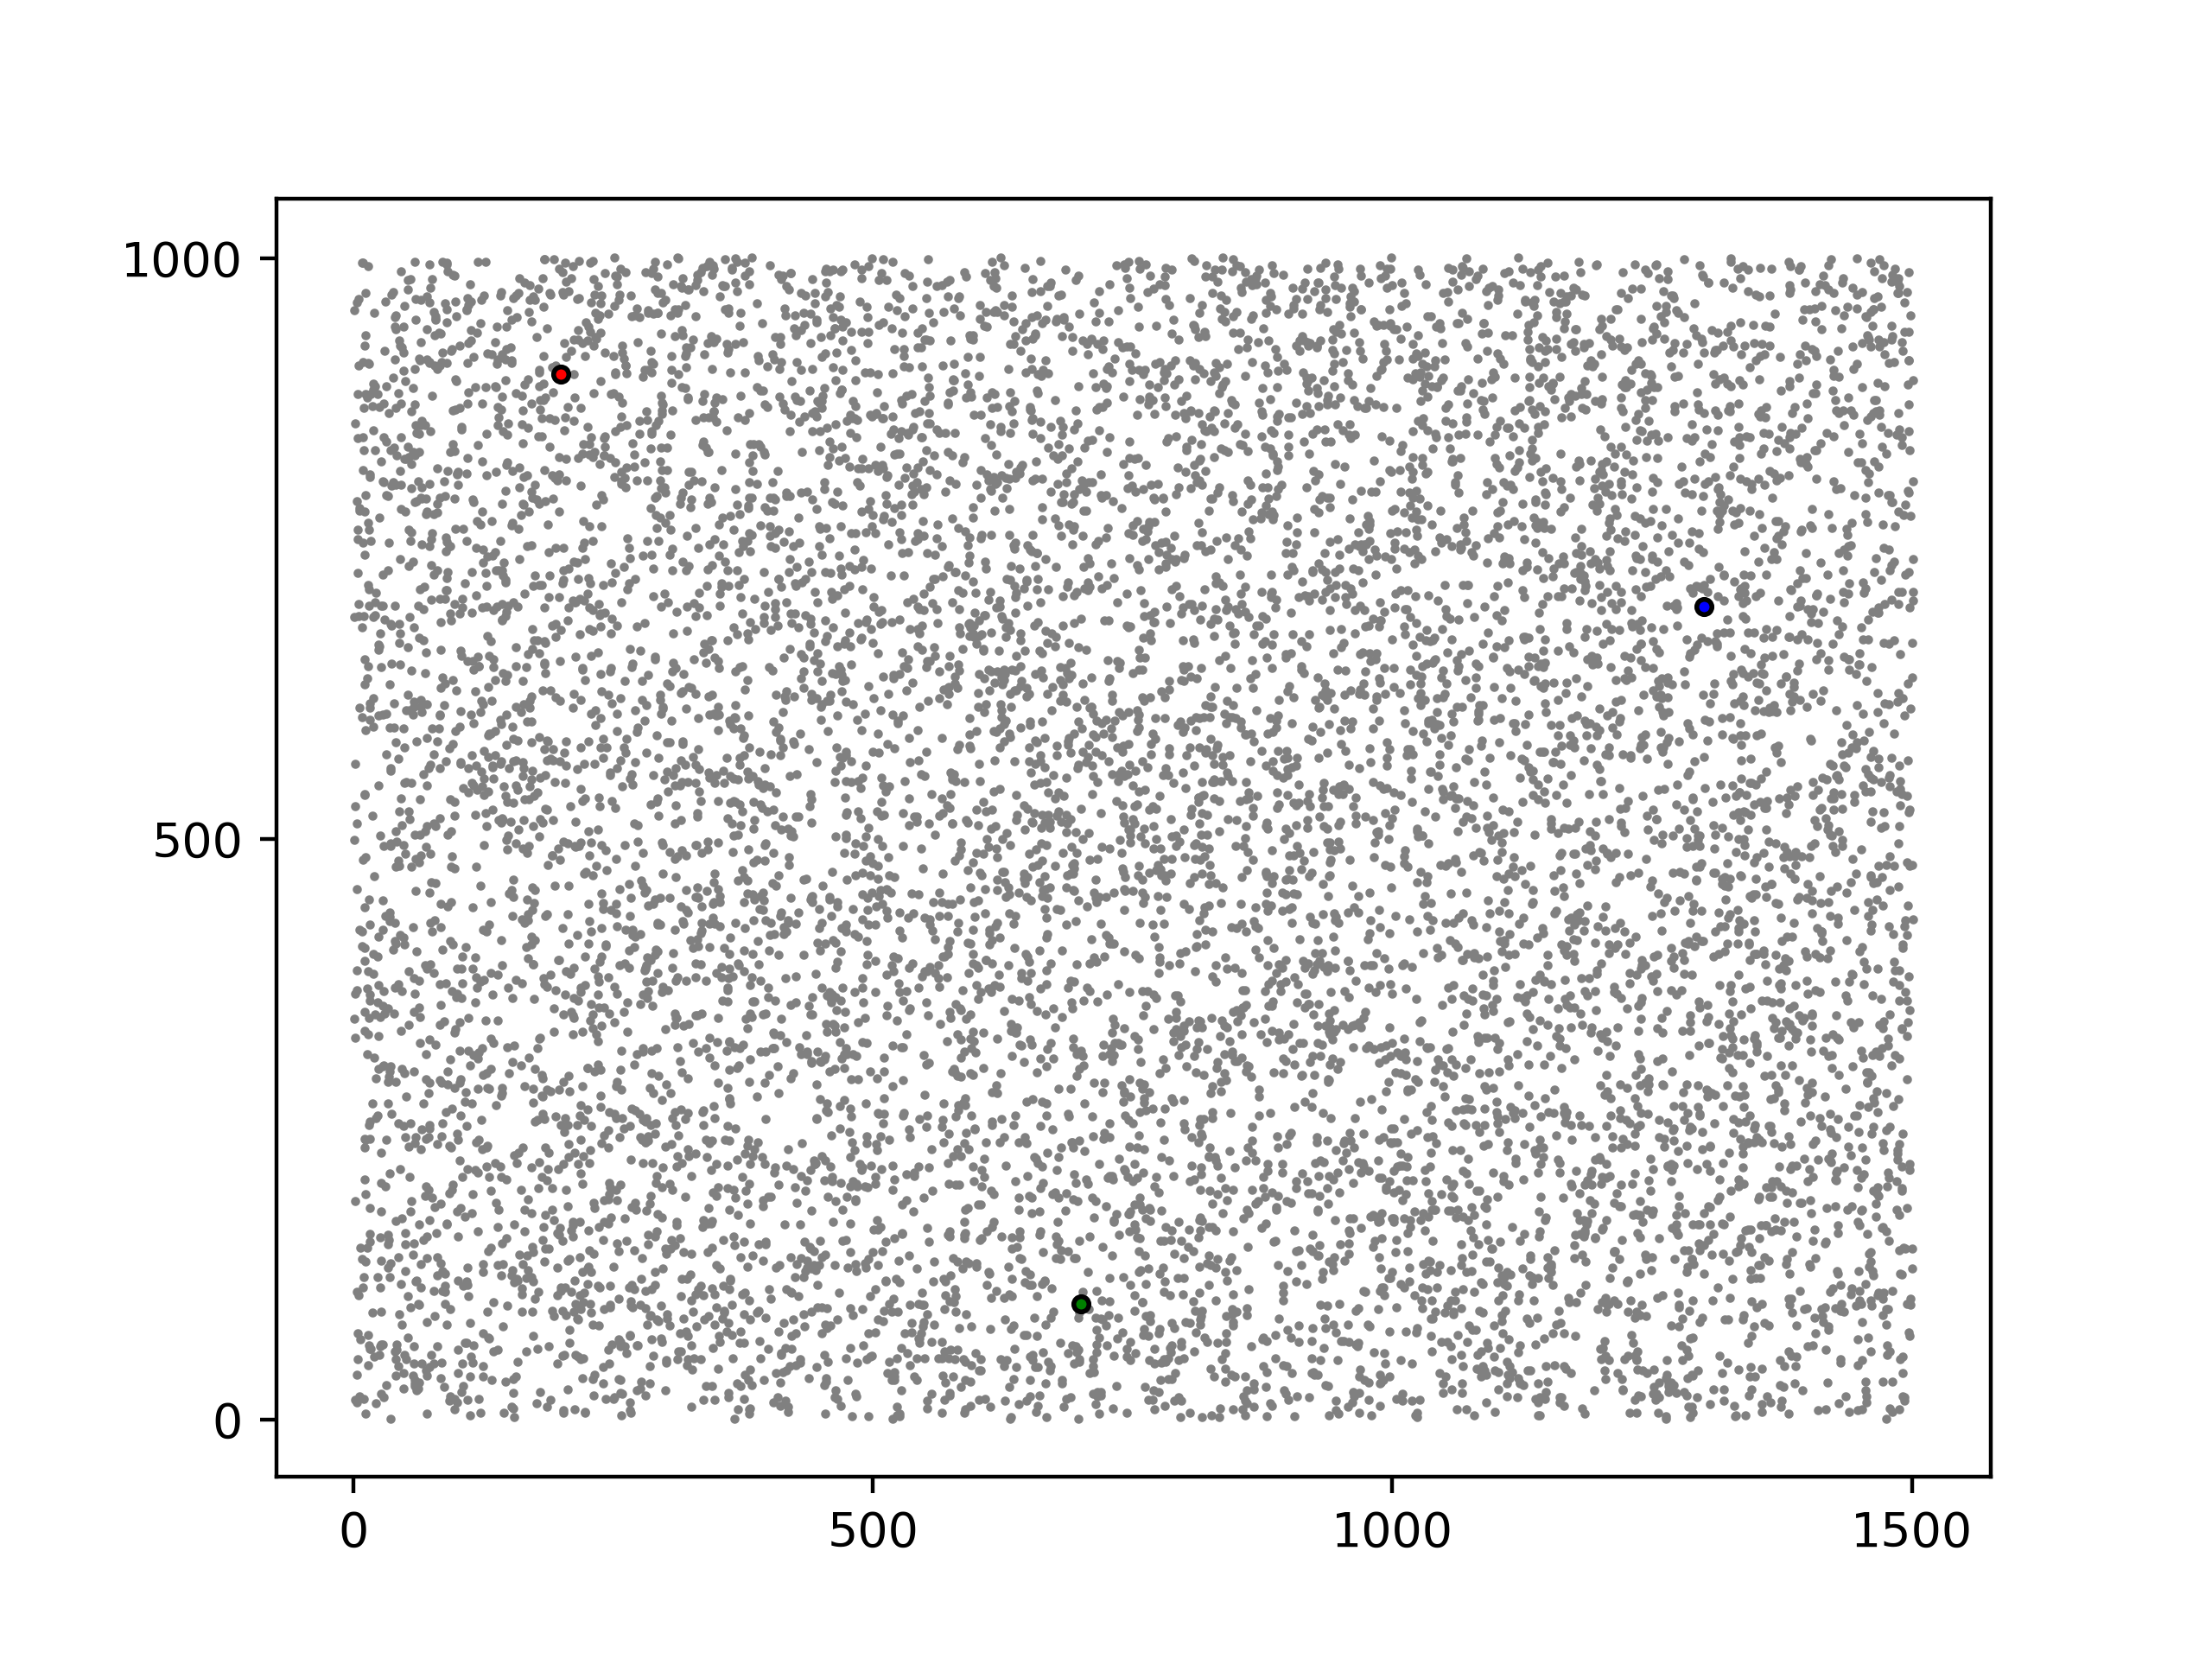
\includegraphics[width=\linewidth]{document/chapters/chapter_7/images/computation_start.png}
    \caption{Computation - Starting point}
    \label{fig:computation_start}
\end{figure}

\begin{figure}[!ht]
    \centering
    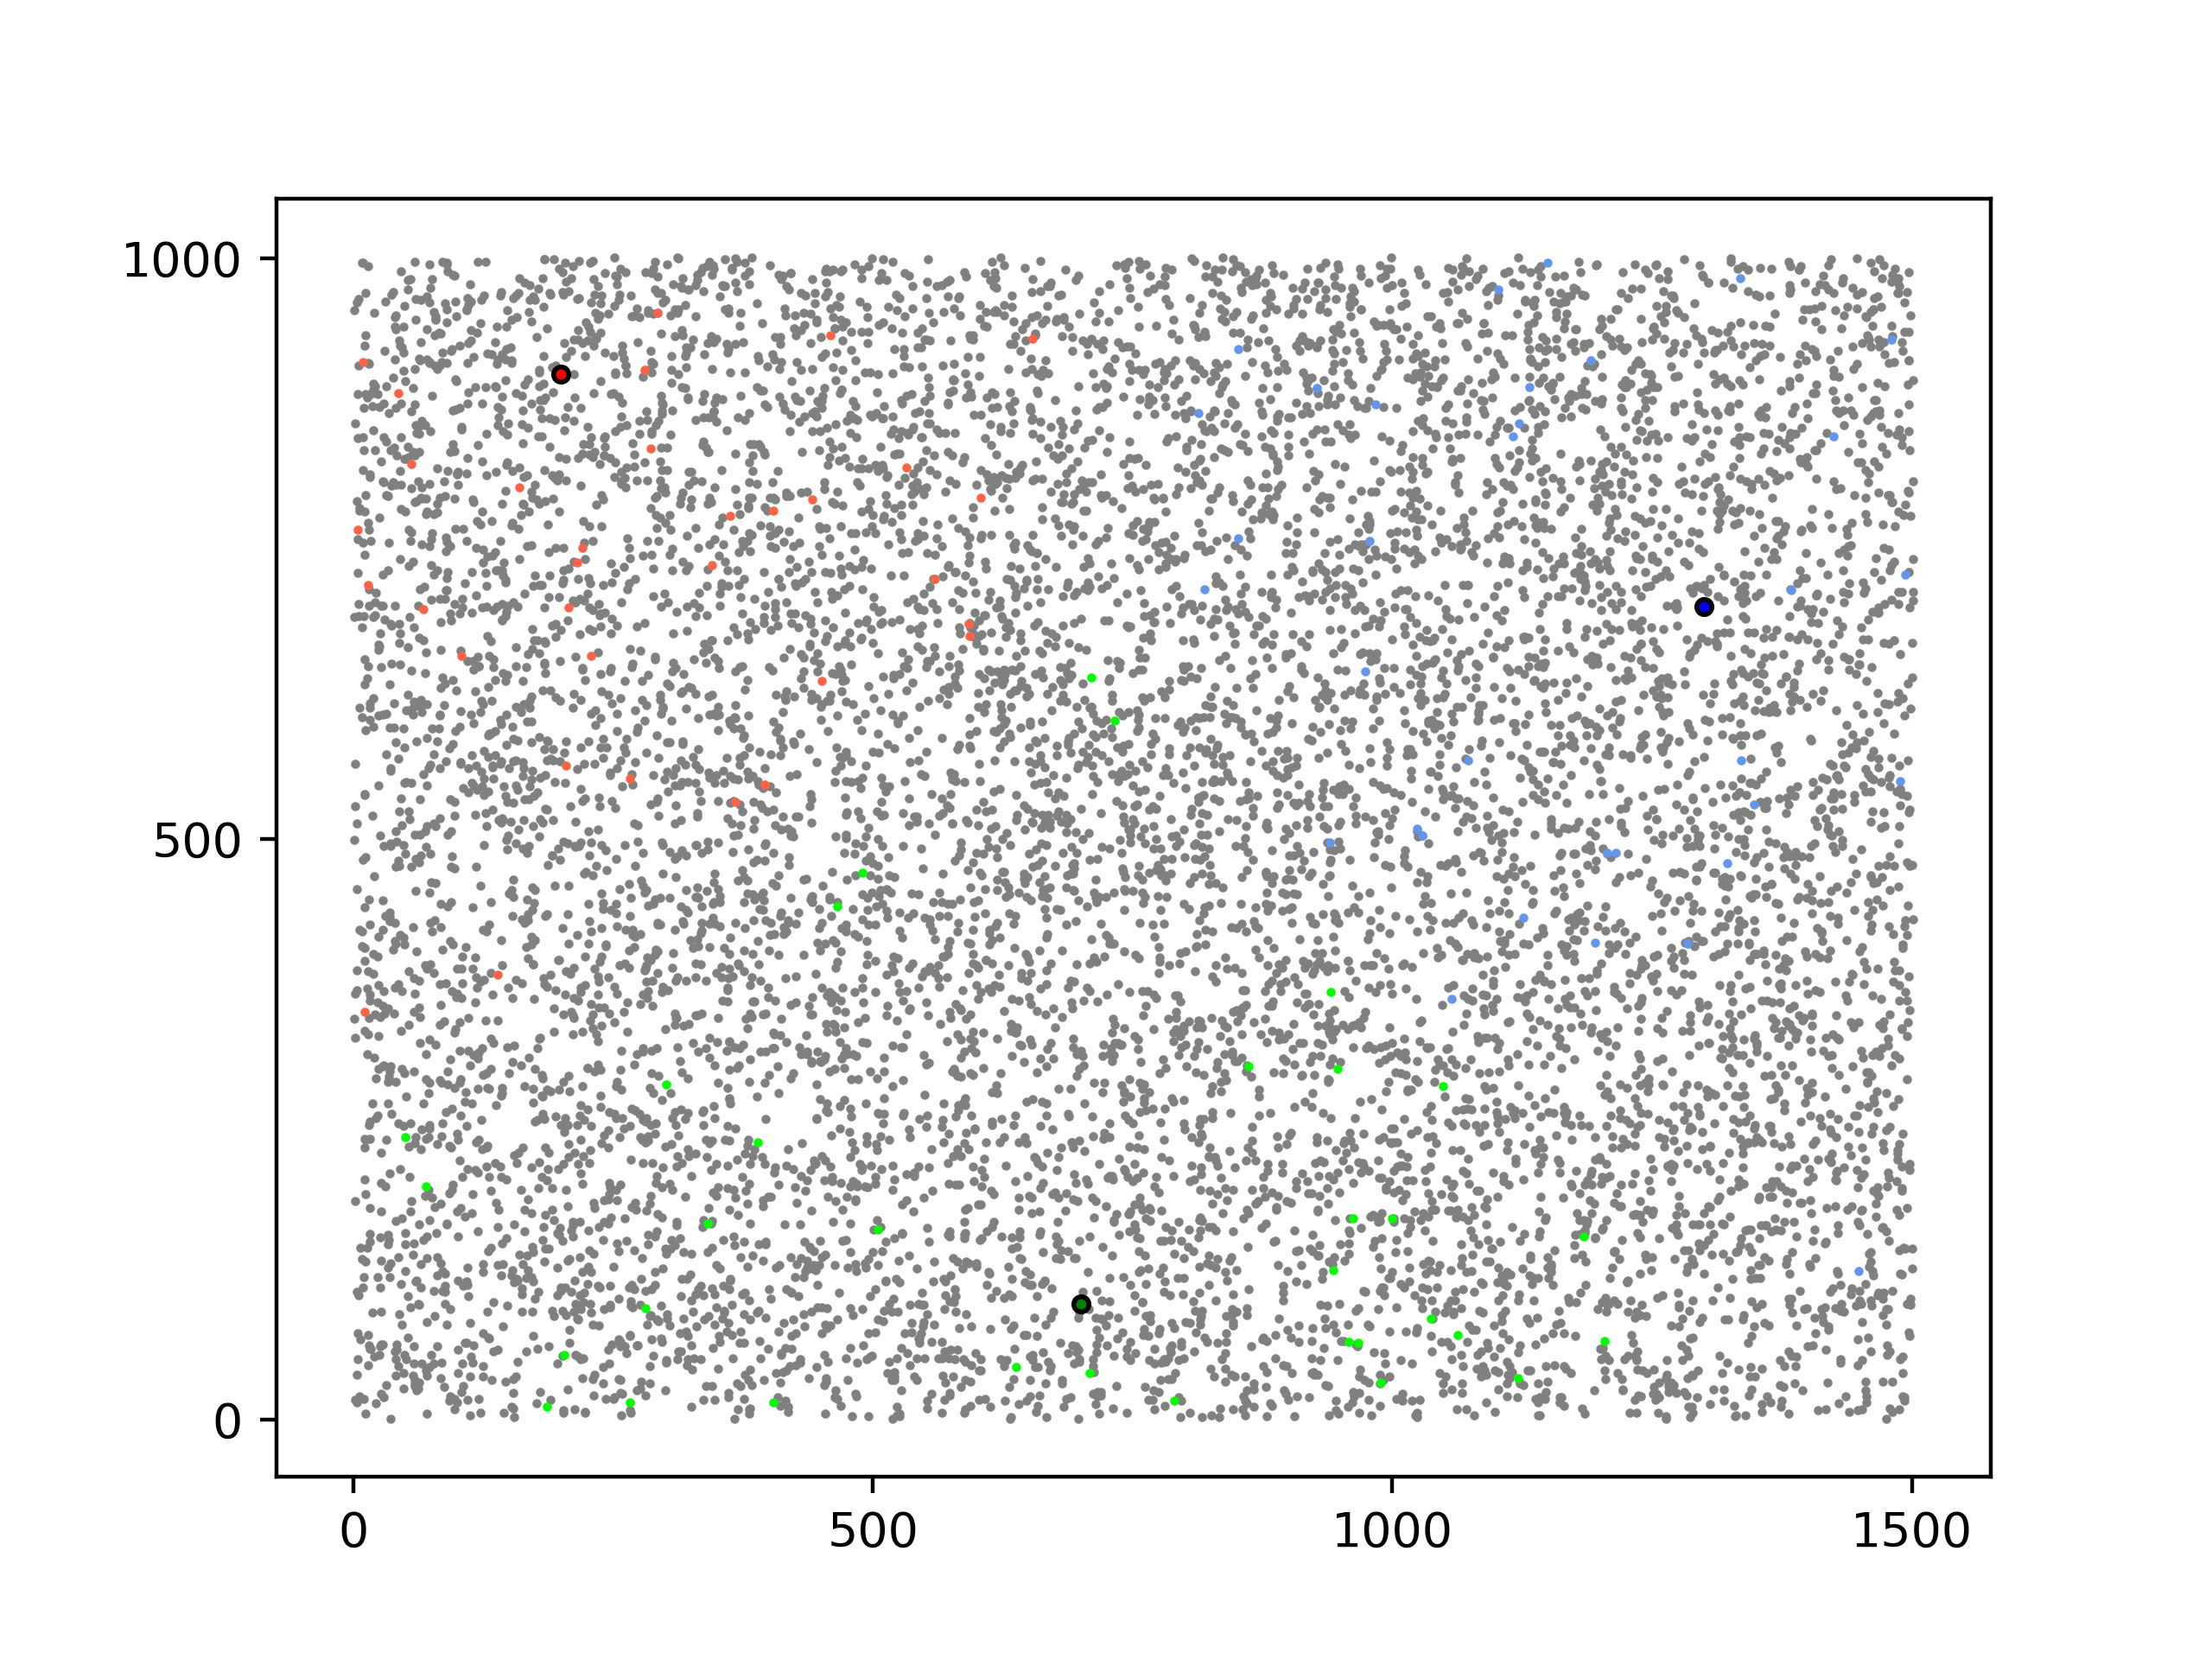
\includegraphics[width=\linewidth]{document/chapters/chapter_7/images/computation_region_computation.png}
    \caption{Computation - Region computation}
    \label{fig:computation_region_computation}
\end{figure}

\begin{figure}[!ht]
    \centering
    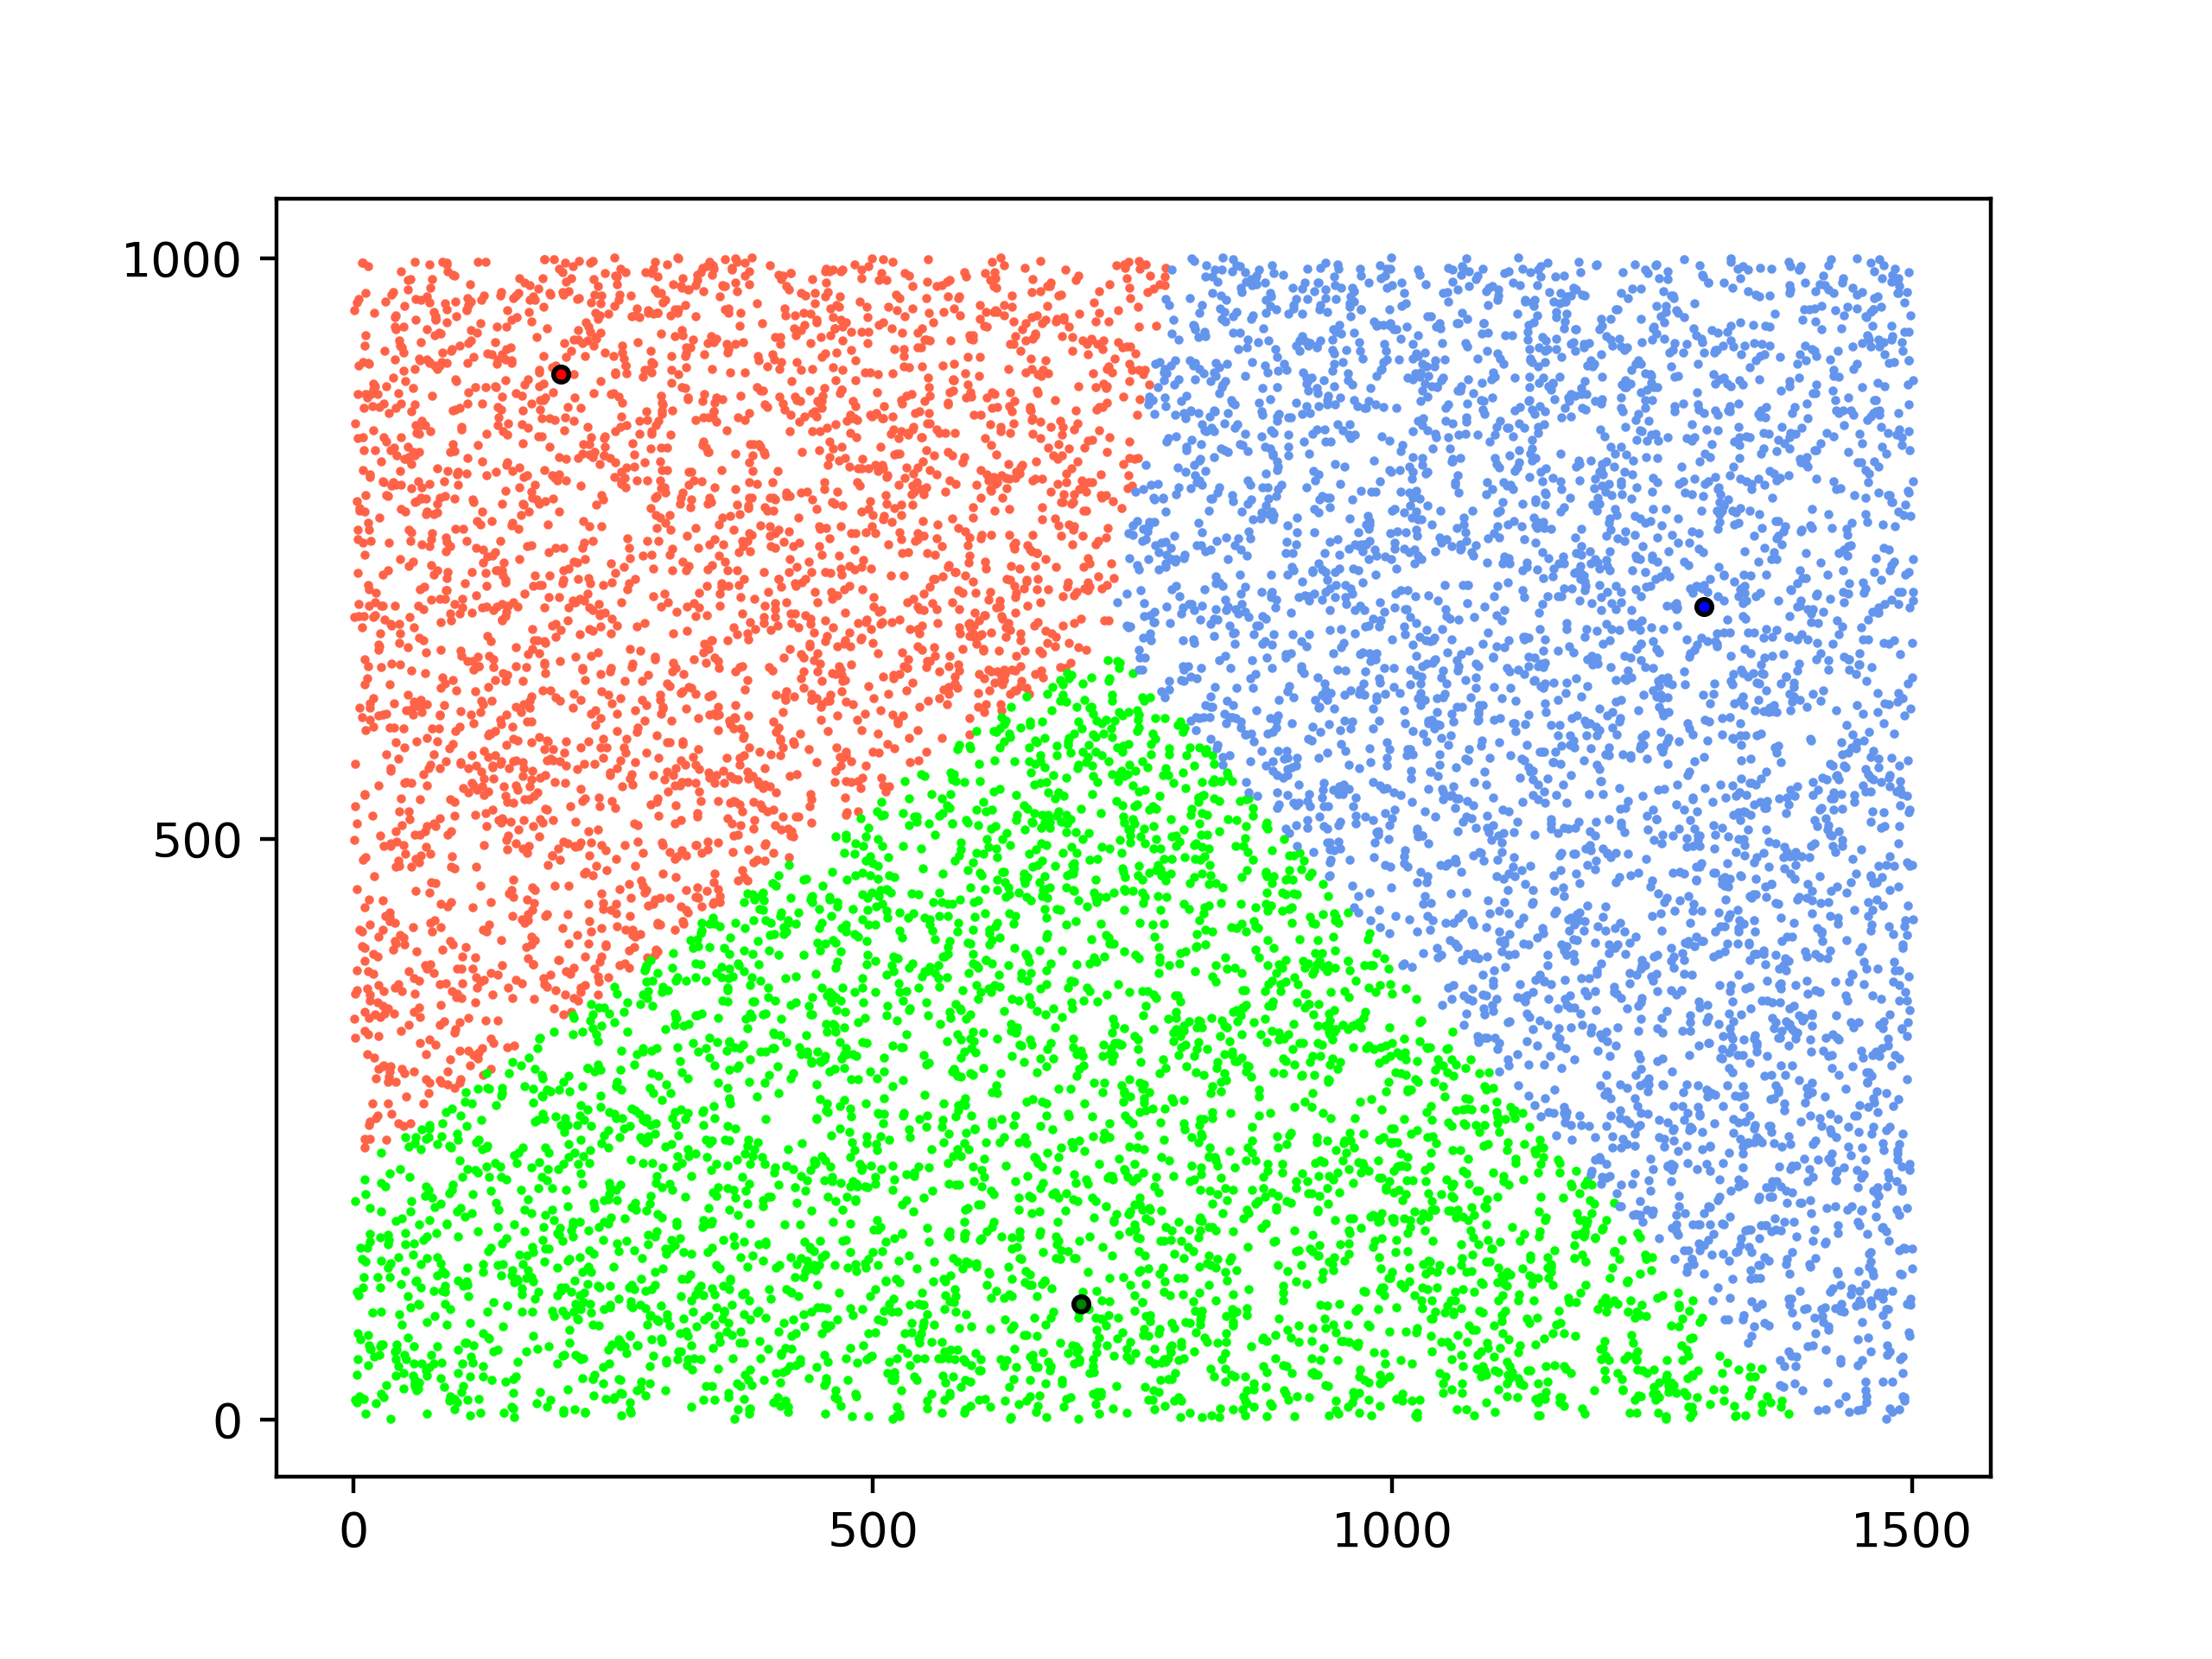
\includegraphics[width=\linewidth]{document/chapters/chapter_7/images/computation_final_result.png}
    \caption{Computation - Final result}
    \label{fig:computation_final_result}
\end{figure}

\subsection{Setup}

\begin{figure}[!ht]
    \centering
    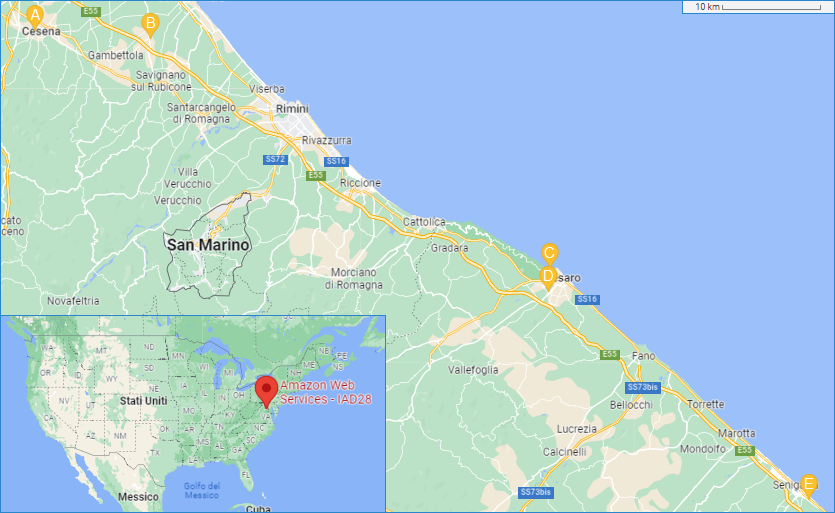
\includegraphics[width=\linewidth]{document/chapters/chapter_7/images/experiment_devices_setup.png}
    \caption{Devices setup}
    \label{fig:experiment_devices_setup}
\end{figure}

\subsection{Results}
TODO

\begin{figure}[!ht]
    \centering
    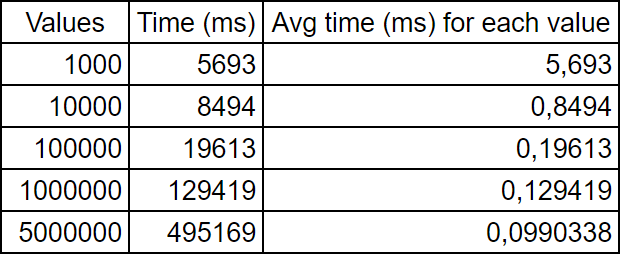
\includegraphics[scale=0.55]{document/chapters/chapter_7/images/experiment_results.png}
    \caption{Experiment results}
    \label{fig:experiment_results}
\end{figure}

\begin{figure}[!ht]
    \centering
    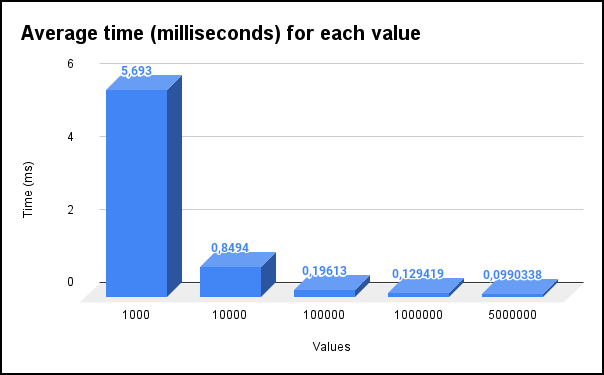
\includegraphics[scale=0.55]{document/chapters/chapter_7/images/experiment_results_avg_ms_per_value.png}
    \caption{Average time (milliseconds) for each value}
    \label{fig:experiment_results_avg_ms_per_value}
\end{figure}